\section{Implementation}
\label{sec:impl}

\name is implemented as a shallow extension of GHC Haskell and runs on top of
Cassandra, an off-the-shelf eventually consistent distributed data (or backing)
store responsible for all data management issues (i.e., replication, fault
tolerance, availability, and convergence).  Template Haskell is used to
implement static contract classification, and proof obligations are discharged
with the help of the Z3~\cite{Z3} SMT solver. Figure~\ref{fig:impl_mod}
illustrates the overall system architecture.

\begin{figure}
\begin{center}
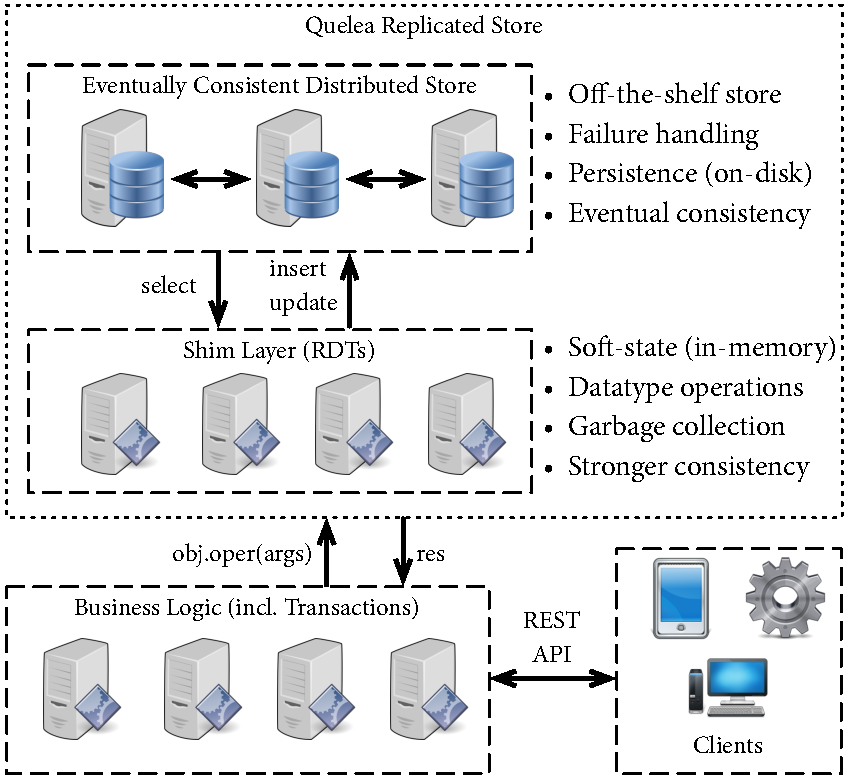
\includegraphics[width=\columnwidth]{Figures/ImplModel}
\end{center}
\caption{Implementation Model.}
\label{fig:impl_mod}
\end{figure}

Replicated data types and various consistency semantics are implemented and
enforced in the \emph{shim layer}. Our implementation supports eventual,
causal, and strong consistency for data type operations, and RC, MAV, and RR
semantics for transactions.  This functionality is implemented entirely on
top of the standard interface exposed by Cassandra. From an engineering
perspective, leveraging an off-the-shelf data store enables an
implementation comprising roughly only 2500 lines of Haskell code, which is
packaged as a library.

\subsection{Operation Consistency}

The shim layer maintains a causally consistent in-memory snapshot of a subset
of objects in the backing store, by explicitly tracking dependencies introduced
between effects due to visibility, session and same transaction relations.
Dependence tracking is similar to the techniques presented in~\cite{BoltOn}
and~\cite{Eiger}. Because Cassandra provides durability, convergence, and fault
tolerance, each shim layer node simply acts as a soft-state cache, with no
inter-node communication, and can safely be terminated at any point. Similarly,
new shim layer nodes can be spawned on demand.

Each effect generated as a result of an effectful operation on an object
inserts a new row $(o,\allowbreak e,\allowbreak txn,\allowbreak val,
\allowbreak deps)$ into the backing store, where $o$ and $e$ are object and
\emph{unique} effect identifiers, $txn$ is an optional transaction identifier,
and $val$ is the value associated with the effect (eg: \cf{Withdraw 50}).
$deps$ is the set of identifiers of \emph{dependencies} of this operation and
is defined as $deps(e) = \{e_1 \ALT \vis{e_1}{e} \wedge \neg(\exists
e_2.\vis{e_1}{e_2} \wedge \vis{e_2}{e})\}$. At any shim layer node, an effect
is included only if all of its dependencies are also included in that node.
This ensures that the state maintained by the shim layer node is causally
consistent. Hence, our dependence tracking strategy ensures that \name does not
track every effect as the number of writes in the system grows.

The shim layer nodes periodically fetch updates from the backing store for
eventually consistent operations, and on-demand for causally consistent and
strongly consistent operations. Strongly consistent operations are performed
after obtaining exclusive leases on objects. The lease mechanism is implemented
with the help of Cassandra's support for conditional updates and expiring
columns.

\subsection{Transactions}

Cassandra does not provide general-purpose transactions. Since the transaction
guarantees provided by \name are coordination-free~\cite{BailisHAT}, we realize
efficient implementations by explicitly tracking dependencies between
operations and transactions. Importantly, the weaker isolation semantics of
transactions in \name permit transactions to be discharged if at least one shim
layer node is reachable.

\begin{figure}
\begin{center}
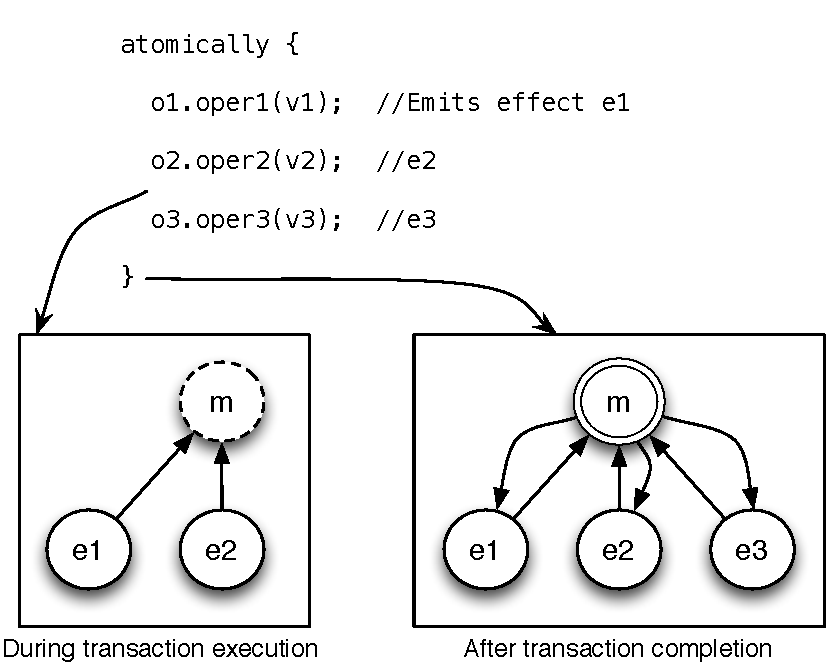
\includegraphics[width=0.8\columnwidth]{Figures/AtomicityImpl}
\end{center}
\caption{Implementing atomicity semantics.}
\label{fig:atomicity_impl}
\end{figure}

\name implements atomic visibility by exploiting shim layer causality
guarantees -- an effect is included only if all the effects if depends on are
also included. Consider the example given in Figure~\ref{fig:atomicity_impl}.
In the figure, the graphs represent the state of the store, where the circles
represent effects and the edges represent the dependence between effects. The
dotted circle represents effects that are not yet inserted into the store.
The graph on the left shows that state of the store after executing \cf{oper2}.
For every transaction in \name, we instantiate a special transaction marker
effect $m$ that is importantly not inserted into the backing store. Marker $m$
is included as a dependence to every effect generated in the transaction. Since
the causally preceding effect $m$ has not yet been written to the store, no
operation will witness $e1$ and $e2$ while the transaction in progress. After
the transaction has finished execution, we insert $m$ into the backing store,
marking all the effects from the transactions as a dependence for $m$, as shown
in the graph on the right. Now, any replica which includes one of the effects
from the transaction must include $m$, and transitively must include every
effect from the transaction. This ensures atomicity and satisfies the RC
requirement.

The above scheme prevents a transaction from witnessing its own effects. This
might conflict with causality requirements on the operations. Hence,
transactions piggy-back the previous effects from the same transaction for each
request. MAV semantics is implemented by keeping track of the set of
transaction markers $M$ witnessed by the transaction, and before performing an
operation at some replica, ensuring that $M$ is a subset of the transaction
markers included at that replica. If not, the missing effects are synchronously
fetched. RR semantics is realized by capturing a optimized snapshot of the
state of some replica; each operation from an RR transaction is applied to this
snapshot state. Any generated effects are added to this snapshot.

\subsection{Summarization}

We utilize the \cf{summarize} function (\S~\ref{sec:summarize}) to summarize
the object state both in the shim layer node and the backing store, typically
when the number of effects on an object crosses a tunable threshold.
Shim layer summarization is straight-forward; a summarization thread takes the
local lock on the cached object, and replaces its state with the summarized
state. The shim layer node only remains unavailable for that particular object
during summarization (usually a few milliseconds).

Performing summarization in the backing store is more complicated since the
whole process needs to be atomic from a client's perspective, but Cassandra
does not provide multi-row transactions. Summarization in the backing store
involves deleting previously inserted rows and inserting new rows, where each
row corresponds to an effect. It is essential that concurrent client operations
are permitted, but are not allowed to witness the intermediate state of the
summarization process.

\begin{figure}
\begin{center}
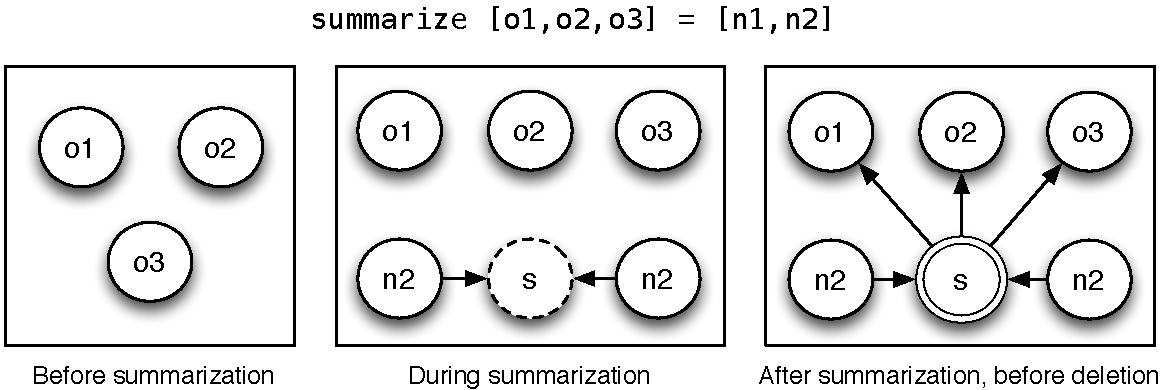
\includegraphics[width=\columnwidth]{Figures/SumDisk}
\end{center}
\caption{Summarization in the backing store.}
\label{fig:impl_sum_disk}
\end{figure}

To this end, we adopt a novel summarization strategy that builds on the
causality property of the store. Figure~\ref{fig:impl_sum_disk} illustrates the
summarization strategy. Suppose the original set of effects on an object are
$o1$, $o2$ and $o3$. When summarized, the new effects yielded are $n1$ and
$n2$. We first instantiate a summarization marker $s$, and similar to
transaction marker, we do not insert it into the store immediately. We insert
the new effects $n1$ and $n2$, with strong consistency, including $s$ as a
dependence. Since $s$ is not yet in the store, the new effects are not made
visible to the clients. Then we insert $s$ with strong consistency, including
the original effects $o1$, $o2$ and $o3$ as dependence. Strongly consistent
insertions ensure that a shim layer node witnessing $s$ on some object must
also witness $n1$ and $n2$ on the same object. A shim layer node which
witnesses all the effects removes the original effects from its cache since
they are superseded by the new effects. Finally, the old effects are deleted
from the backing store. This process ensures that clients either witness the
old or the new effects, but not both; the summarization process appears to be
atomic from the clients perspective.
